% задание и сама лабораторная работа
% Для листинга кода:
\lstset{ %
	language=C,                % Язык программирования                % где поставить нумерацию строк (слева\справа)
	numberstyle=\tiny,           % размер шрифта для номеров строк
	stepnumber=1,                   % размер шага между двумя номерами строк
	numbersep=5pt,                % как далеко отстоят номера строк от подсвечиваемого кода
	showspaces=false,            % показывать или нет пробелы специальными отступами
	showstringspaces=false,      % показывать или нет пробелы в строках
	showtabs=false,             % показывать или нет табуляцию в строках
	tabsize=2,                 % размер табуляции по умолчанию равен 2 пробелам
	captionpos=t,              % позиция заголовка вверху [t] или внизу [b] 
	breaklines=true,           % автоматически переносить строки (да\нет)
	breakatwhitespace=false,       
	frame=single,                    % Добавить рамку
	basicstyle=\small,
	escapebegin=\begin{russian}\commentfont,
		escapeend=\end{russian},
	literate={Ö}{{\"O}}1
	{Ä}{{\"A}}1
	{Ü}{{\"U}}1
	{ß}{{\ss}}1
	{ü}{{\"u}}1
	{ä}{{\"a}}1
	{ö}{{\"o}}1
	{~}{{\textasciitilde}}1
	{а}{{\selectfont\char224}}1
	{б}{{\selectfont\char225}}1
	{в}{{\selectfont\char226}}1
	{г}{{\selectfont\char227}}1
	{д}{{\selectfont\char228}}1
	{е}{{\selectfont\char229}}1
	{ё}{{\"e}}1
	{ж}{{\selectfont\char230}}1
	{з}{{\selectfont\char231}}1
	{и}{{\selectfont\char232}}1
	{й}{{\selectfont\char233}}1
	{к}{{\selectfont\char234}}1
	{л}{{\selectfont\char235}}1
	{м}{{\selectfont\char236}}1
	{н}{{\selectfont\char237}}1
	{о}{{\selectfont\char238}}1
	{п}{{\selectfont\char239}}1
	{р}{{\selectfont\char240}}1
	{с}{{\selectfont\char241}}1
	{т}{{\selectfont\char242}}1
	{у}{{\selectfont\char243}}1
	{ф}{{\selectfont\char244}}1
	{х}{{\selectfont\char245}}1
	{ц}{{\selectfont\char246}}1
	{ч}{{\selectfont\char247}}1
	{ш}{{\selectfont\char248}}1
	{щ}{{\selectfont\char249}}1
	{ъ}{{\selectfont\char250}}1
	{ы}{{\selectfont\char251}}1
	{ь}{{\selectfont\char252}}1
	{э}{{\selectfont\char253}}1
	{ю}{{\selectfont\char254}}1
	{я}{{\selectfont\char255}}1
	{А}{{\selectfont\char192}}1
	{Б}{{\selectfont\char193}}1
	{В}{{\selectfont\char194}}1
	{Г}{{\selectfont\char195}}1
	{Д}{{\selectfont\char196}}1
	{Е}{{\selectfont\char197}}1
	{Ё}{{\"E}}1
	{Ж}{{\selectfont\char198}}1
	{З}{{\selectfont\char199}}1
	{И}{{\selectfont\char200}}1
	{Й}{{\selectfont\char201}}1
	{К}{{\selectfont\char202}}1
	{Л}{{\selectfont\char203}}1
	{М}{{\selectfont\char204}}1
	{Н}{{\selectfont\char205}}1
	{О}{{\selectfont\char206}}1
	{П}{{\selectfont\char207}}1
	{Р}{{\selectfont\char208}}1
	{С}{{\selectfont\char209}}1
	{Т}{{\selectfont\char210}}1
	{У}{{\selectfont\char211}}1
	{Ф}{{\selectfont\char212}}1
	{Х}{{\selectfont\char213}}1
	{Ц}{{\selectfont\char214}}1
	{Ч}{{\selectfont\char215}}1
	{Ш}{{\selectfont\char216}}1
	{Щ}{{\selectfont\char217}}1
	{Ъ}{{\selectfont\char218}}1
	{Ы}{{\selectfont\char219}}1
	{Ь}{{\selectfont\char220}}1
	{Э}{{\selectfont\char221}}1
	{Ю}{{\selectfont\char222}}1
	{Я}{{\selectfont\char223}}1
	{і}{{\selectfont\char105}}1
	{ї}{{\selectfont\char168}}1
	{є}{{\selectfont\char185}}1
	{ґ}{{\selectfont\char160}}1
	{І}{{\selectfont\char73}}1
	{Ї}{{\selectfont\char136}}1
	{Є}{{\selectfont\char153}}1
	{Ґ}{{\selectfont\char128}}1
}

\newpage
\section*{Задание}
\addcontentsline{toc}{section}{\tocsecindent{Задание}}
\subsection*{Постановка задачи}
\addcontentsline{toc}{subsection}{\tocsecindent{Постановка задачи}}
Реализовать загружаемый модуль ядра, выводящий информацию о процессах.


\subsection*{Листинг кода}
\addcontentsline{toc}{subsection}{\tocsecindent{Листинг кода}}
\begin{lstlisting}[language=c,caption=Листинг кода заголовочного файла]
#ifndef STACK_H
#define STACK_H

#include <stdio.h>
#include <stdlib.h>
#include <string.h>
#define NMAX 100000

struct elem 
{
	char *filename;
	int len;
};

struct stack 
{
	struct elem elems[NMAX];
	int top;
};

void init(struct stack *stk);
void push(struct stack *stk, char *filename, int len);
struct elem pop(struct stack *stk);
int isempty(struct stack *stk);

#endif
\end{lstlisting}
\begin{lstlisting}[language=c,caption=Листинг кода программы]
#include <sys/stat.h>
#include <dirent.h>
#include <stdio.h>
#include <string.h>
#include <unistd.h>
#include <string.h>
#include <errno.h>
#include "stack.h"

#define	FTW_F	1 
#define	FTW_D	2	
#define	FTW_DNR	3	
#define	FTW_NS 4

typedef	int	AnyType(const char *, int, int);

static AnyType myFunc;
static int myFtw(char *, AnyType *);
static int doPath(AnyType *, char*, int);
static struct stack stk;

void init(struct stack *stk) 
{
	stk->top = 0;
}

void push(struct stack *stk, char *filename, int len)
{
	if (stk->top < NMAX)
	{
		stk->elems[stk->top].filename = calloc(strlen(filename), sizeof(char));
		strcpy(stk->elems[stk->top].filename, filename);
		stk->elems[stk->top].len = len;
		stk->top++;
	} 
	else
		printf("Стек полон!\n");
}

struct elem pop(struct stack *stk)
{
	struct elem el;
	if ((stk->top) > 0)
	{
		stk->top--;
		el.filename = calloc(strlen(stk->elems[stk->top].filename), sizeof(char));
		strcpy(el.filename, stk->elems[stk->top].filename);
		free(stk->elems[stk->top].filename);
		el.len = stk->elems[stk->top].len;
		
		return el;
	}
	else
	{
		printf("Стек пуст!\n");
		return el;
	}
}

int isempty(struct stack *stk) 
{
	if(stk->top == 0)
		return 1;
	else
		return 0;
}

static int myFtw(char *pathname, AnyType *func)
{
	if (chdir(pathname) == -1)
	{
		printf("Ошибка вызова функции chdir %s\n", pathname);
		return 1;
	}

	init(&stk);
	push(&stk, ".", 0);

	while (!isempty(&stk)) 
	{
		struct elem el = pop(&stk);
		doPath(func, el.filename, el.len);
	}
	
	return 0;
}

static int doPath(AnyType* func, char *fullpath, int len)
{
	if (len < 0)
	{
		if (chdir(fullpath) == -1)
		{
			printf("Каталога не существует!");
			return 1;
		}
	
		return 0;
	}
	
	struct stat	statbuf;
	struct dirent	*dirp;
	DIR	*dp;

	if (lstat(fullpath, &statbuf) == -1)	
	{
		return 1;
	}

	if (S_ISDIR(statbuf.st_mode) == 0)
	{
		return 1;
	}

	func(fullpath, FTW_D, len);

	if ((dp = opendir(fullpath)) == NULL)
	{
		return 1;
	}


	if (chdir(fullpath) == -1)
	{
		printf("Ошибка вызова функции chdir %s\n", fullpath);
		return 1;
	}

	len += 5;
	
	push(&stk, "..", -1);
	while ((dirp = readdir(dp)) != NULL)
	{
		if (strcmp(dirp->d_name, ".") != 0 && strcmp(dirp->d_name, "..") != 0 && strcmp(dirp->d_name, ".git") != 0)
		{
			push(&stk, dirp->d_name, len);
		}
	}

	if (closedir(dp) == -1)
		printf("Невозможно закрыть каталог %s\n", fullpath);

	return 0;
}

static int myFunc(const char *pathname, int type, int len)
{
	if (type == FTW_D)
	{
		for (int i = 0; i < len; i++)
		{
			if (i % 5 == 1 && i / 5 != 0)
				printf("|");
			else
				printf(" ");
		}
		
	printf(" |- %s\n", pathname);
	}

	return 0;
}

int main(int argc, char *argv[])
{
	if (argc != 2)
	{
		printf("Не указан <начальный_каталог!>\n");
		return 1;
	}

return myFtw(argv[1], myFunc); 
}
\end{lstlisting}
\section*{Результат работы}
\addcontentsline{toc}{subsection}{\tocsecindent{Результат работы}}
1. Скомпилируем программу и продемонстрируем вывод дерева каталогов, задав начальным каталог "∼/"
\begin{figure}[h!]
\center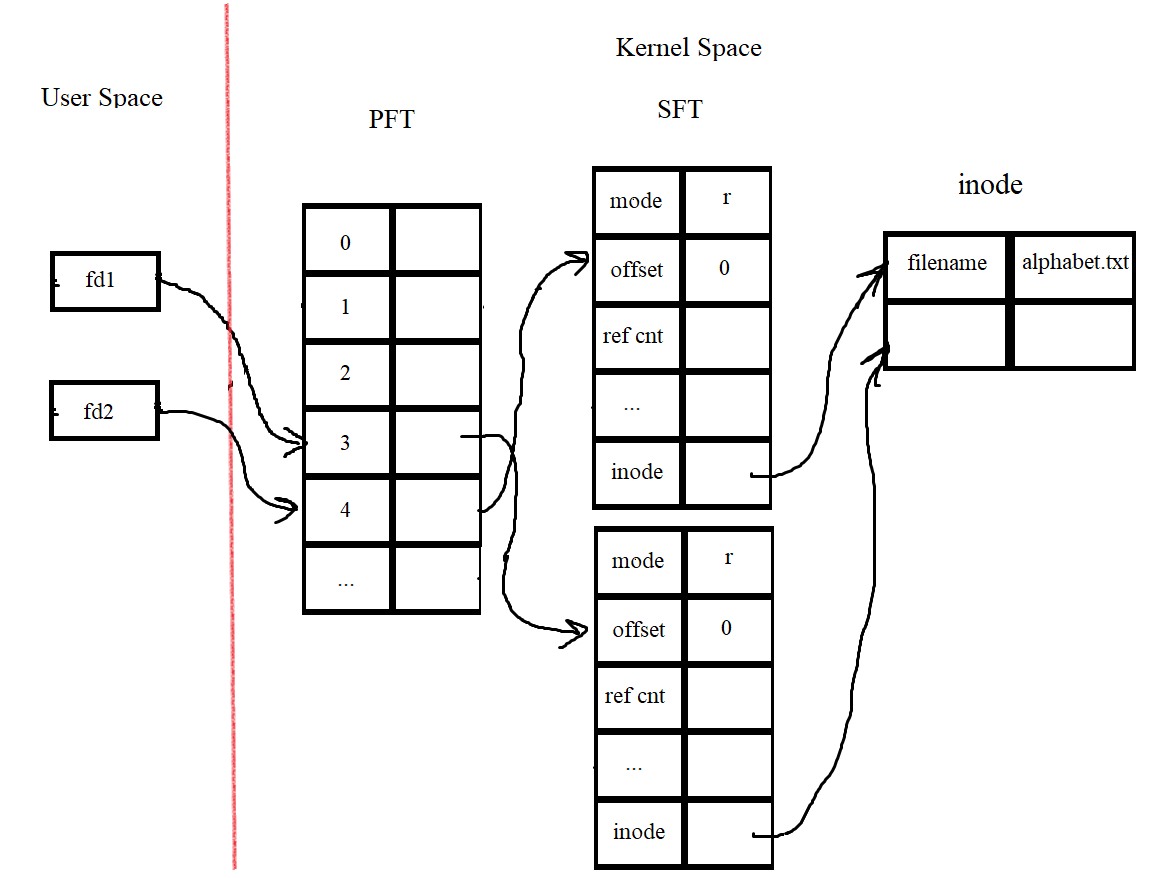
\includegraphics[scale=0.75]{2.png}
\end{figure}
\begin{figure}[h!]
\center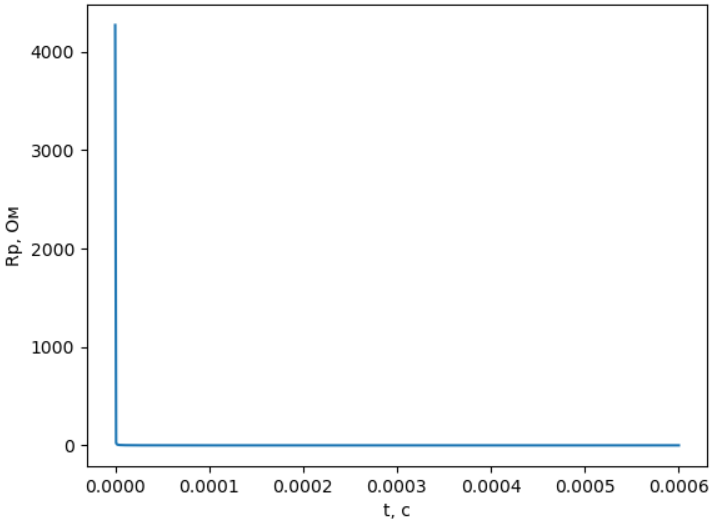
\includegraphics[scale=0.75]{3.png}
\end{figure}
\newpage
\begin{figure}[h!]
	\center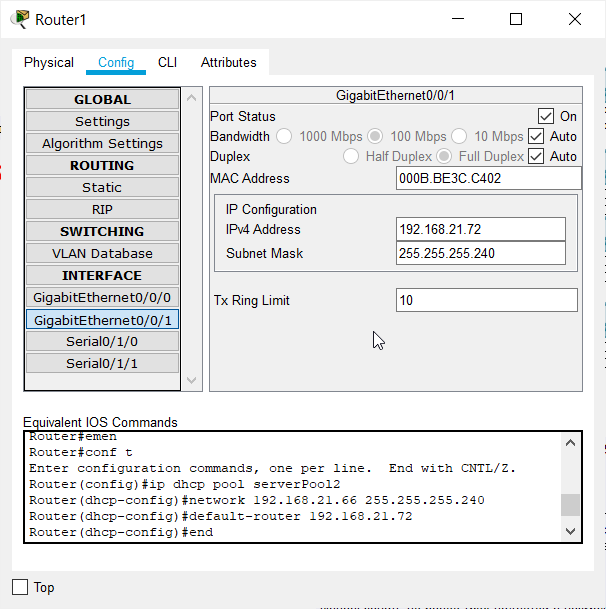
\includegraphics[scale=0.7]{4.png}
\end{figure}
\begin{figure}[h!]
	\center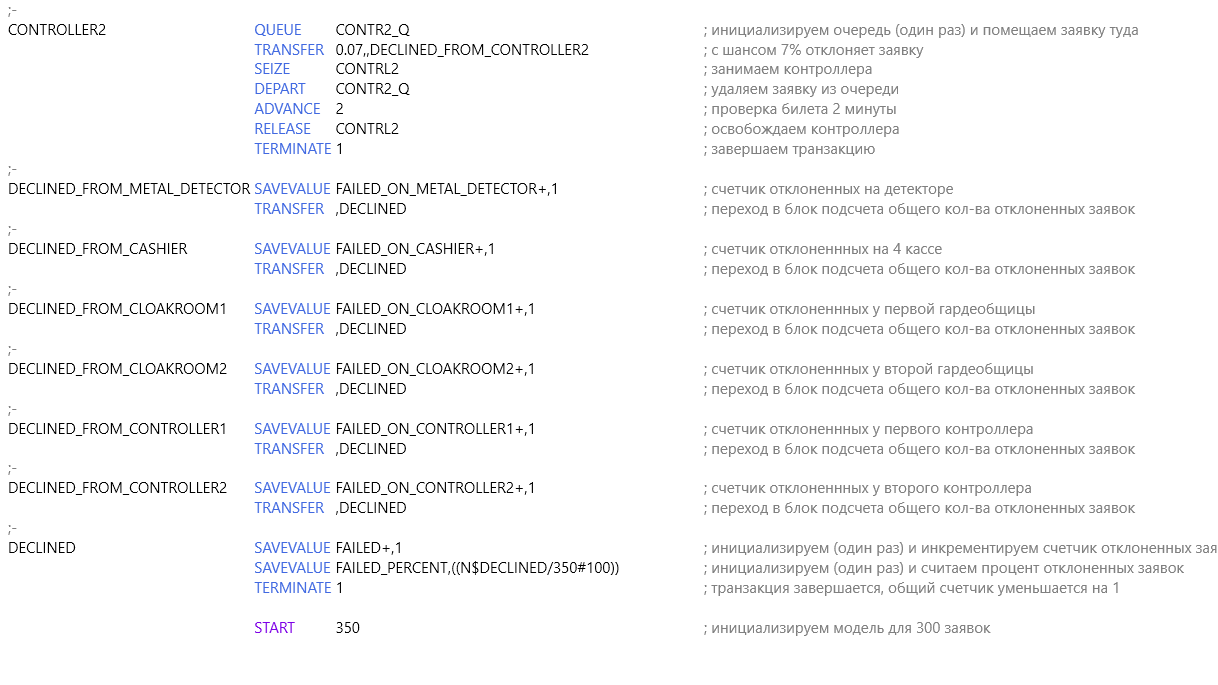
\includegraphics[scale=0.7]{5.png}
\end{figure}
\begin{figure}[h!]
	\center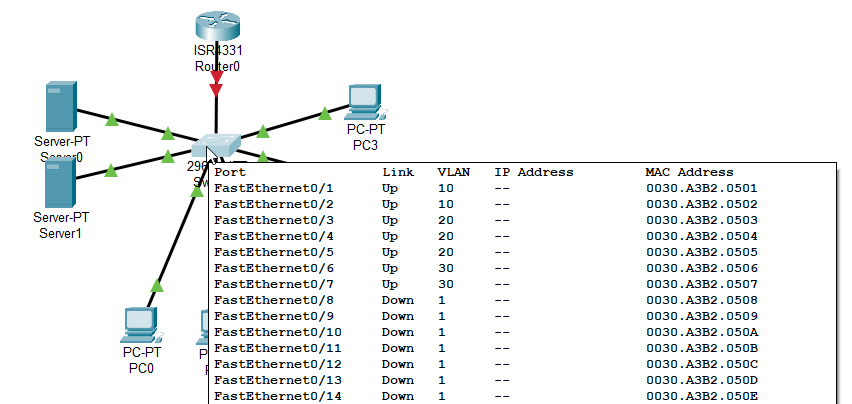
\includegraphics[scale=0.7]{6.png}
\end{figure}
\newpage
2. Покажем ошибочные ситуации: запуск без указания начального каталога и с указанием несуществующего каталога.
\begin{figure}[h!]
	\center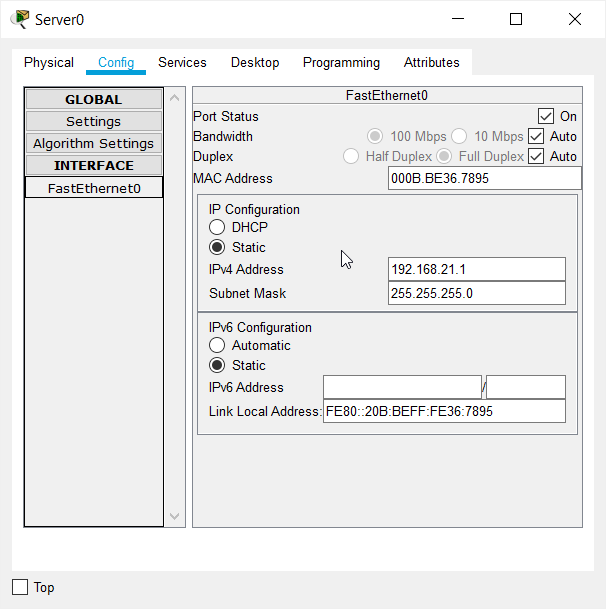
\includegraphics[scale=1]{1.png}
\end{figure}
\begin{figure}[h!]
	\center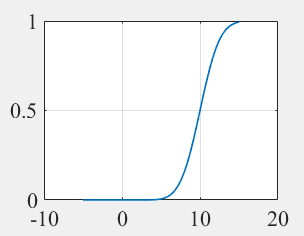
\includegraphics[scale=1]{7.png}
\end{figure}
\newline 3. Комментарии к программе:
\begin{itemize}
	\item После обработки всех файлов в каталоге вызывается функция chdir(“...”), чтобы использовать короткие имена.
	\item Функция stat() заполняет структуру struct stat информацией об определенном файле; если при этом необходимо обнаруживать символьные ссылки, следует использовать lstat()
	\item Условиями выхода из рекурсии служат следующие ситуации: \begin{enumerate}
	\item произошла ошибка вызова stat,\item тип файла не является каталогом,\item вызываемый
	каталог не доступен,\item ошибкa вызова функции chdir(),\item а также возврат 0 в конце функции.
\end{enumerate}
\item Функция opendir(const char *name) открывает директорию для чтения с именем
name и возвращает указатель на поток директории. Функция closedir(DIR *dirp)
закрывает директорию для чтения.
\item chdir(const char *path) - функция смены рабочего каталога. Она устанавливает
текущий каталог, указанный в аргументе path.
\item Функция lstat(const char *file\_name, struct stat *buf) возвращает информацию о
файле, заданном с помощью file\_name и заполняет буфер buf. Она может возвращать следующие ошибки:\begin{enumerate}
\item EBADF (неверный файловый дескриптор filedes);
\item EFAULT (некорректный адрес);
\item ENOENT (компонент полного имени файла file\_name не существует или полное имя является пустой строкой);

\item ELOOP (при поиске файла встретилось слишком много символьных ссылок);
\item ENOTDIR (компонент пути не является каталогом);
\item ENOMEM (недостаточно памяти в системе);
\item EACCES (доступ запрещен);

\item ENAMETOOLONG (слишком длинное имя файла).	\end{enumerate}
\end{itemize}
